\documentclass[tikz,border=5pt]{standalone}
\usepackage[UTF8]{ctex}
\usepackage{amsmath,amssymb}
\usetikzlibrary{arrows.meta,calc,angles,quotes}
\definecolor{MotionBlue}{HTML}{245A81}
\definecolor{MotionRed}{HTML}{9F3C31}
\tikzset{axis/.style={-{Stealth[length=2mm]},thin},vec/.style={-{Stealth[length=2.5mm]},very thick,MotionBlue},aux/.style={dashed,gray},every node/.style={font=\small}}
\begin{document}

% geometry-01: actual fixed-radius tangent geometry, counterclockwise motion.
\begin{tikzpicture}[scale=1.25]
\coordinate(O) at (0,0);\coordinate(H) at (3.4,0);\coordinate(T) at (.85,1.472243);
\draw[gray!60] (O) circle(1.7);
\draw[axis] (-1.95,0)--(4.05,0) node[right]{$x$};
\draw[axis] (0,-1.95)--(0,2.25) node[above]{$y$};
\draw[thick] (O)--(T) node[midway,left]{$r$};
\draw[aux] (T)--(H);
\draw[vec] (T)--(-.09,2.015) node[above left]{$\boldsymbol v_T$};
\draw[MotionRed,thick] (.985,1.394)--(.907,1.259)--(.772,1.337);
\draw[axis,MotionBlue] (-1.47,.85) arc(150:195:1.7) node[midway,left]{$\omega$};
\draw[<->] (0,-.38)--(3.4,-.38) node[midway,fill=white]{$l$};
\draw (.48,0) arc(0:60:.48) node[midway,right]{$\theta$};
\fill (O) circle(1.2pt) node[below left]{$O$};
\fill (H) circle(1.7pt) node[below right]{$H$};
\fill (T) circle(1.7pt) node[right]{$T$};
\node at (1,-2.45){$\boldsymbol v_T\parallel HT,\quad OT\perp HT$};
\end{tikzpicture}

% projection-01: rotating basis anchored at the moving rider.
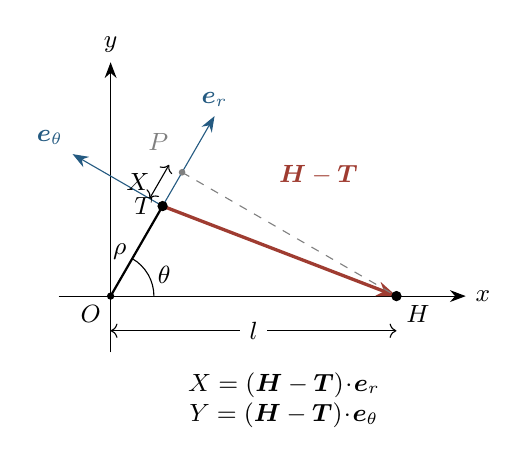
\begin{tikzpicture}[scale=1.1]
\coordinate(O) at (0,0);\coordinate(T) at (.6,1.03923);
\coordinate(P) at(.825,1.42894);
\coordinate(H) at (3.3,0);
\draw[axis] (-.6,0)--(4.1,0) node[right]{$x$};
\draw[axis] (0,-.65)--(0,2.7) node[above]{$y$};
\draw[thick] (O)--(T) node[midway,left]{$\rho$};
\draw[axis,MotionBlue] (T)--(1.2,2.07846) node[above]{$\boldsymbol e_r$};
\draw[axis,MotionBlue] (T)--(-.43923,1.63923) node[above left]{$\boldsymbol e_\theta$};
\draw[vec,MotionRed] (T)--(H);
\node[MotionRed] at(2.4,1.4){$\boldsymbol H-\boldsymbol T$};
\draw[aux] (P)--(H);
\fill[gray] (P) circle(1.1pt);
\node[gray] at(.55,1.78){$P$};
\draw[<->] (.45,1.12583)--(.675,1.51554) node[midway,left]{$X$};
\draw (.5,0) arc(0:60:.5) node[midway,right]{$\theta$};
\draw[<->] (0,-.4)--(3.3,-.4) node[midway,fill=white]{$l$};
\fill (O) circle(1.2pt) node[below left]{$O$};
\fill (T) circle(1.7pt) node[left]{$T$};
\fill (H) circle(1.7pt) node[below right]{$H$};
\node[align=center] at (2,-1.2){$X=(\boldsymbol H-\boldsymbol T)\!\cdot\!\boldsymbol e_r$\\$Y=(\boldsymbol H-\boldsymbol T)\!\cdot\!\boldsymbol e_\theta$};
\end{tikzpicture}

% cardioid-01: ground axes centered at O; H is fixed at l>r.
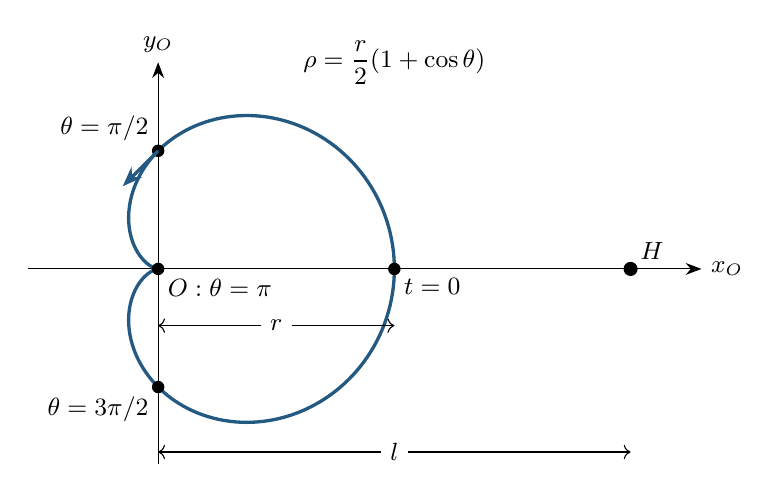
\begin{tikzpicture}[scale=1.5]
\draw[axis] (-1.1,0)--(4.6,0) node[right]{$x_O$};
\draw[axis] (0,-1.65)--(0,1.75) node[above]{$y_O$};
\draw[very thick,MotionBlue,samples=240,domain=0:360] plot({(1+cos(\x))*cos(\x)},{(1+cos(\x))*sin(\x)});
\fill (2,0) circle(1.5pt) node[below right]{$t=0$};
\fill (0,1) circle(1.5pt) node[above left]{$\theta=\pi/2$};
\fill (0,-1) circle(1.5pt) node[below left]{$\theta=3\pi/2$};
\fill (0,0) circle(1.5pt) node[below right]{$O:\theta=\pi$};
\fill (4,0) circle(1.7pt) node[above right]{$H$};
\draw[vec] (0,1)--(-.3,.7);
\draw[<->] (0,-1.55)--(4,-1.55) node[midway,fill=white]{$l$};
\draw[<->] (0,-.48)--(2,-.48) node[midway,fill=white]{$r$};
\node at (2,1.75){$\rho=\dfrac r2(1+\cos\theta)$};
\end{tikzpicture}

% ellipse-01: axes are centered at T, not at the ellipse center C.
\begin{tikzpicture}[scale=.75]
\draw[axis] (-4.65,0)--(3,0) node[right]{$X$};
\draw[axis] (0,-4.65)--(0,4.8) node[above]{$Y$};
\draw[aux] (-1,-4.35)--(-1,4.35);
\draw[very thick,MotionBlue] (-1,0) ellipse[x radius=3,y radius=4];
\fill (0,0) circle(1.7pt) node[below right]{$T$};
\fill (-1,0) circle(1.5pt) node[below left]{$C$};
\fill (2,0) circle(1.7pt) node[above right]{$\theta=0$};
\fill (-4,0) circle(1.7pt) node[below left]{$\theta=\pi$};
\fill (-1,-4) circle(1.7pt) node[below]{$\theta=\pi/2$};
\fill (-1,4) circle(1.7pt) node[above]{$\theta=3\pi/2$};
\draw[vec] (1.853,-1.236)--(1.63,-1.94);
\draw[<->] (-1,.5)--(0,.5) node[midway,above]{$r/2$};
\draw[<->] (-1,-1)--(2,-1) node[midway,fill=white]{$l-r/2$};
\draw[<->] (-4.45,0)--(-4.45,4) node[midway,left]{$l$};
\node at (-.8,-5.4){$C=(-r/2,0)$，轨迹按顺时针方向遍历};
\end{tikzpicture}

% polar-01: exact velocity components on the left, acceleration on the right.
\begin{tikzpicture}[scale=1.05]
\begin{scope}
\coordinate(O) at(0,0);\coordinate(T) at(.75,1.299038);
\draw[aux] (O)--(T);
\draw[axis] (T)--(1.25,2.165) node[above]{$\boldsymbol e_r$};
\draw[axis] (T)--(-.116,1.799) node[above left]{$\boldsymbol e_\theta$};
\draw[vec,MotionRed] (T)--(.49,.849) node[midway,right]{$\dot\rho\boldsymbol e_r$};
\draw[vec] (.49,.849)--(-.289,1.299);
\node[MotionBlue] at(-.5,.7){$\rho\omega\boldsymbol e_\theta$};
\draw[vec,black] (T)--(-.289,1.299) node[midway,above]{$\boldsymbol v_T$};
\fill (O) circle(1.5pt) node[below]{$O$};\fill (T) circle(1.5pt) node[right]{$T$};
\node at (.4,-.55){速度的径向与切向分解};
\end{scope}
\begin{scope}[xshift=5cm]
\coordinate(O) at(0,0);\coordinate(T) at(.75,1.299038);
\draw[aux] (O)--(T);
\draw[axis] (T)--(1.25,2.165) node[above]{$\boldsymbol e_r$};
\draw[axis] (T)--(-.116,1.799) node[above left]{$\boldsymbol e_\theta$};
\draw[vec,MotionRed] (T)--(.15,.2598) node[midway,left]{$a_r$};
\draw[vec] (.15,.2598)--(1.05,-.2598) node[midway,below]{$a_\theta$};
\draw[vec,black] (T)--(1.05,-.2598) node[midway,right]{$\boldsymbol a_T$};
\fill (O) circle(1.5pt) node[below left]{$O$};\fill (T) circle(1.5pt) node[right]{$T$};
\node at(.4,-.85){$a_r=\ddot\rho-\rho\omega^2$};
\node at(.4,-1.35){$a_\theta=2\omega\dot\rho$};
\end{scope}
\end{tikzpicture}

% rates-01: different measured speeds, same physical time and same r,w.
\begin{tikzpicture}[x=3.3cm,y=1.7cm]
\draw[axis] (0,0)--(2.2,0) node[right]{$\theta/\pi$};
\draw[axis] (0,0)--(0,2.45) node[above]{$|\boldsymbol v|/(r\omega)$};
\foreach\x in{0.5,1,1.5,2}{\draw(\x,0)--(\x,-.04) node[below]{$\x$};}
\foreach\y in{1,1.5,2}{\draw(0,\y)--(-.025,\y) node[left]{$\y$};}
\draw[aux] (1,0)--(1,2.1);
\draw[MotionBlue,very thick,samples=180,domain=0:2] plot(\x,{abs(cos(90*\x))});
\draw[MotionRed,very thick,samples=180,domain=0:2] plot(\x,{sqrt(2.25*sin(180*\x)^2+4*cos(180*\x)^2)});
\node[MotionBlue] at(.5,.32){地面观察};
\node[MotionRed] at(1,2.22){木马旋转坐标观察};
\node at(1,-.57){示例：$l=2r$，$\theta=\omega t$};
\end{tikzpicture}
\end{document}
